%% ------------------------------------------------------------------------- %%
\chapter{Development}
\subsection{Parallelization of Ghmatecd and Ghmatece subroutines}
%\label{cap:ghmatec_parallel}
In BEM, it is necessary to create four matrices, two for the static problem and 
two for the dynamic problem. In the static problem, those two matrices $H$ and $G$
are real, but in the dynamic problem, they are complex. Analysing the algorithm
provided by (Carrion), it is possible to conclude that the time complexity
to generate $H$ and $G$ for one problem is $\Theta(N \times NBE \times NPG^2)$,
thus a huge amount of computational power is required. Since in the dynamic problem
those matricies are all complex, the constant associated with the asymptotic time
complexity are even higher than the static problem, requiring even more
computational power.

Let's focus on the static problem first. To generate $H$ and $G$, both real matrices
of dimension $3 \cdot NBE \times 3 \cdot N$, the algorithm provided by (Carrion), 
implemented in Ghmatece, do it in the following way: 
It breaks down $H$ and $G$ in $3 \times 3$ block matrices $H_{ij}$ and $G_{ij}$, 
then runs a $\Theta(NPG^2)$ 
algorithm, for each $1 \leq i \leq NBE$ and $1 \leq j \leq N$. Although the
original code had a call to a procedure that calculates the Gaussian quadrature
for each $H_{ij}$ and $G_{ij}$ block matrix, a dependency analysis show that
it was not necessary; this calculation could be done once and the result passed
as argument to Ghmatece. Thus, there was no dependency between each $H_{ij}$ and
each $G_{ij}$, implying that $H$ and $G$ could be built in a parallel fashion.

Since each $H_{ij}$ and $G_{ij}$ can be computed in parallel and the number of block
columns is higher than the number of cores on a shared memory machine (even for small
instances), an efficient way of parallelizing such computations is to compute all block
columns in parallel. With OpenMP, a simple "parallel do" clause is enough 
(check lines 95-96).

Using the technique described above to compute $H$ and $G$ on a GPU would result 
in a waste of resources because a GPU can do much more calculations in parallel, but
with a lower sequential performance. In order to build both matrices on these devices,
it is better to generate all $H_{ij}$ and $G_{ij}$ in parallel. For that, allocate a block for 
each $H_{ij}$ and $G_{ij}$, and unroll the Nonsinge procedure (ignoring the Singular case) 
in order to allocate one thread for each $NPG^2$.In the end, there will be $NBE \times N$ 
blocks and $NPG \times NPG$ threads. 

Since Nonsinge creates a matrix of dimension $3 \times 3$ 
per $NPG^2$ and sums them all, a buffer is needed to hold all matrices before casting
a reduction, otherwise, a race condition would appear. Allocating such buffer in shared 
memory is a good idea because it is faster than global memory and enables a small degree 
of parallelism in the final reduction wihout needing to launch a new kernel.

Remember that the singular case was ignored in the above analysis. Since the singular
case is only responsible for generating the main diagonal of those matrices, and the
calculations are somewhat different from the nonsingular case, then it can be generated in
the CPU in parallel and the result merged with the ones obtained in the GPU. Of course, those
calculations can also be computed in a different kernel and merged together with the results
from the kernel responsible for the nonsingular case, but tests are needed to verify which one
is faster. 

For the dynamic version of the problem, its parallelization is very similar to the static version,
but the computations in the singular and nonsingular case are almost the same so that doing or not
doing the first case in the same kernel as the second yielded the same time results (see lines 
218-219 of kernels/Ghmatecd\_cu.cu). Later, the main diagonal of the dynamic problem matrices 
must be summed with the main diagonal of the static problem matrices.

\subsection{Parallelization of Interec subroutine}
%\label{cap: interec_parallel}
TODO.

\label{cap:desenvolvimentos}

Um exemplo de figura est� na figura~\ref{fig:graph}.
\begin{figure}[htb]
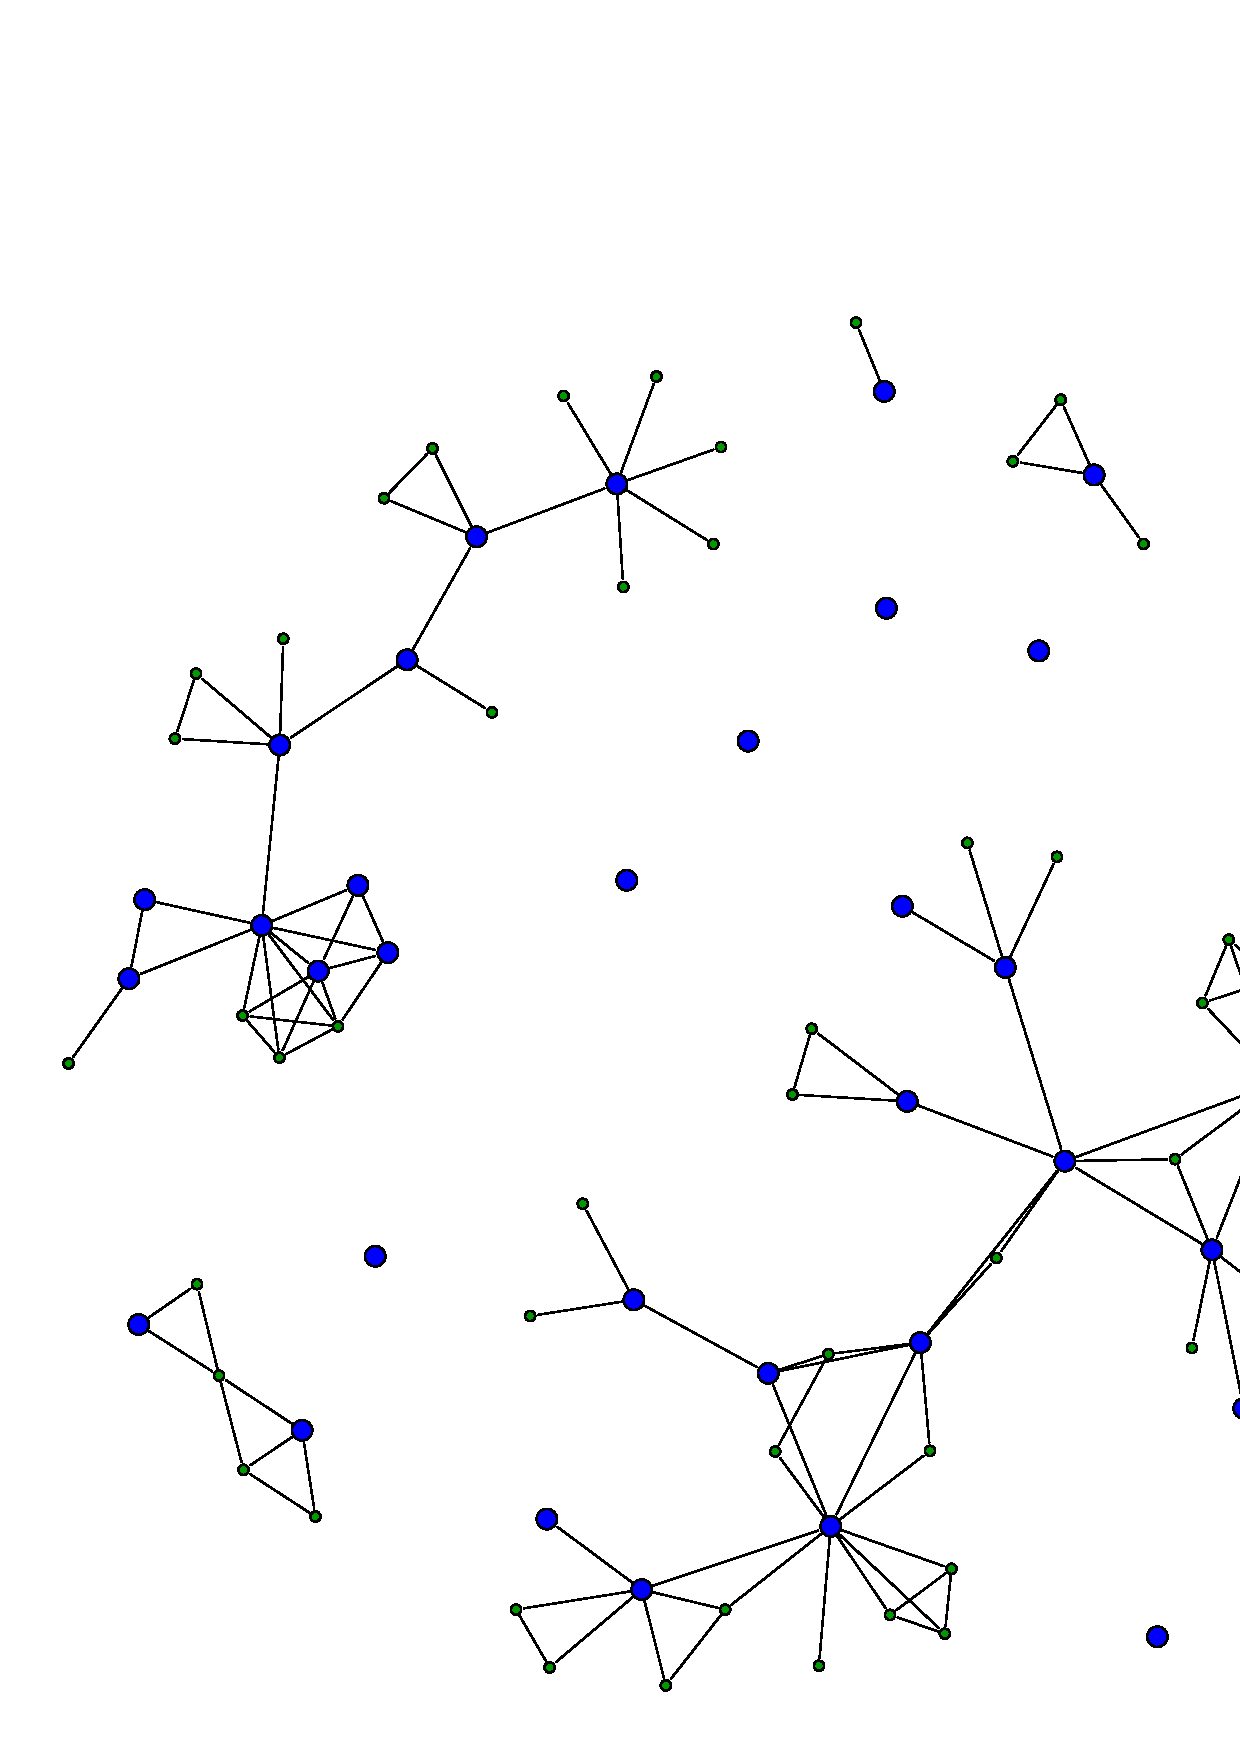
\includegraphics[width=5cm]{figuras/graph}
\caption{\label{fig:graph}Exemplo de uma figura.}
\end{figure}
